\subsection{A mean-field approximation example}
\label{sec:chap2_mean_field_vi}
As an example for the variational inference algorithm, here we present the variational mean-field approximation \citep{parisi:book1988} for Bayesian linear regression. Readers are also referred to \citet{bishop:prml2006} for more details and here we would briefly cover the derivations presented there. Mean-field approximation, also known as the factorised approximation, assumes the approximate posterior to be the form of
\begin{equation}
q(\mparam) := \prod_{i=1}^{D} q_i(\theta_i).
\label{eq:chap2_mean_field}
\end{equation}
In general one can partition the elements of $\mparam = (\theta_1, \theta_2, ..., \theta_D)$ into disjoint groups and apply factorisations over groups. This general case is usually called \emph{structured} mean-field approximation \citep{saul:structured1996}, and for simplicity in the following example we only consider the fully factorised case (\ref{eq:chap2_mean_field}). Also we emphasise that there's no further assumption/restriction that is made on the functional form of $q_i(\theta_i)$. As we shall see, the variational free-energy is still convex in $q_i(\theta_i)$ and thus the solution provided by the following is the global optimum.

To derive the best approximation in the mean-field distribution family, we first substitute (\ref{eq:chap2_mean_field}) into (\ref{eq:chap2_vfe}) (and use $\mparam_{\neq j}$ to denote all the $\theta_i$ variables except $\theta_j$):
\begin{equation*}
\begin{aligned}
\mathcal{F}_{\text{VFE}}(q; p) &=  \int \prod_i q_i(\theta_i)  \left( \sum_{i} \log q_i(\theta_i) - \log p^*(\mparam)  \right) d\mparam \\
&= \int q_j(\theta_j) \log q_j(\theta_j) d\theta_j  - \int q_j(\theta_j) \left( \int \prod_{i \neq j} q_i(\theta_i)  \log p^*(\mparam) d\mparam_{\neq j} \right) d\theta_j + \text{const}\\
&:=  \int q_j(\theta_j) \log q_j(\theta_j) d\theta_j  - \int q_j(\theta_j) \log \tilde{p}(\theta_j) d\theta_j + \text{const},
\end{aligned}
\end{equation*}
where $\tilde{p}(\theta_j)$ denote the ``marginal'' distribution satisfying
\begin{equation*}
\log \tilde{p}(\theta_j) = \int \prod_{i \neq j} q_i(\theta_i) \log p^*(\mparam) d\mparam_{\neq j} + \text{const}.
\end{equation*}
This means, by fixing the functional form of $q_i$ for all $i \neq j$, VFE is reduced to the KL-divergence $\mathrm{KL}[q_j(\theta_j)||\tilde{p}(\theta_j)]$ plus a constant that is independent to $q_j(\theta_j)$. Thus the free-energy is still convex in $q_j(\theta_j)$, in which the unique global optimum is obtained by setting $q_j(\theta_j) = \tilde{p}(\theta_j)$. To be precise, we explicitly write down the optimal mean-field approximation as
\begin{equation}
q_j(\theta_j) = \frac{ \exp \left[ \int \prod_{i \neq j} q_i(\theta_i)  \log p^*(\mparam) d\mparam_{\neq j} \right] }{ \int \exp \left[ \int \prod_{i \neq j} q_i(\theta_i)  \log p^*(\mparam) d\mparam_{\neq j} \right] d\theta_j}.
\label{eq:chap2_mean_field_opt}
\end{equation}
%
Now as an example consider Bayesian linear regression with 2-D inputs $\bm{x}$ and 1-D output $y$:
\begin{equation*}
\mparam \sim \mathcal{N}(\mparam; \bm{\mu}_0, \bm{\Lambda}_0^{-1}), \quad 
y|\bm{x} \sim \mathcal{N}(y; \mparam^T \bm{x}, \sigma^2).
\end{equation*}
Given the observations $\data = \{ (\bm{x}_n, y_n) \}_{n=1}^N$, the posterior distribution of $\mparam$ can be computed analytically as $p(\mparam|\mathcal{D}) = \mathcal{N}(\mparam; \bm{\mu}, \bm{\Lambda}^{-1})$ with $\bm{\Lambda} = \bm{\Lambda}_0 + \frac{1}{\sigma^2} \sum_n \bm{x}_n \bm{x}_n^T$ and $\bm{\Lambda} \bm{\mu} = \bm{\Lambda}_0 \bm{\mu}_0 + \frac{1}{\sigma^2} \sum_n y_n \bm{x}_n$. To see how the mean-field approach works, we explicitly write down the elements of the posterior parameters
\begin{equation*}
\bm{\mu} = \begin{pmatrix} \mu_1 \\ \mu_2 \end{pmatrix}, \quad
\bm{\Lambda} = \begin{pmatrix} \Lambda_{11} & \Lambda_{12} \\ \Lambda_{21} & \Lambda_{22} \end{pmatrix}, 
\quad \Lambda_{12} = \Lambda_{21},
\end{equation*}
Then by explicitly expanding the mean-field solution (\ref{eq:chap2_mean_field_opt}):
\begin{equation}
\begin{aligned}
\log q_1(\theta_1) &= \int q_2 \log p(\mparam, \mathcal{D}) d\theta_2 + \text{const} \\
&= \mathbb{E}_{q_2} \left[ -\frac{1}{2} (\theta_1 - \mu_1)^2 \Lambda_{11} - (\theta_1 - \mu_1) \Lambda_{12} (\theta_2 - \mu_2) \right] + \text{const} \\
&= -\frac{1}{2} \theta_1^2 \Lambda_{11} + \theta_1 \mu_1 \Lambda_{11} - \theta_1 \Lambda_{12} (\mathbb{E}_{q_2}[\theta_2] - \mu_2) + \text{const} \\
&:= \log \mathcal{N}(\theta_1; m_1, \lambda^{-1}) + \text{const}
\end{aligned}
\label{eq:chap2_mean_field_linear_regression}
\end{equation}
where the new mean $m_1$ and the precision $\lambda_1$ satisfies
\begin{equation*}
m_1 = \mu_1 - \Lambda_{11}^{-1}\Lambda_{12} (\mathbb{E}_{q_2}[\theta_2] - \mu_2), \quad
\lambda_1 = \Lambda_{11}.
\end{equation*}
It is important to note again that we do not assume the approximation to be a Gaussian distribution in order to obtain the last equation in (\ref{eq:chap2_mean_field_linear_regression}). Rather the Gaussian distribution solution came out from the derivation of the global optimum (\ref{eq:chap2_mean_field_opt}) and the completion of the square form.
%
One can derive the terms $m_2 = \mu_2 - \Lambda_{22}^{-1}\Lambda_{21} (\mathbb{E}_{q_1}[\theta_1] - \mu_1)$ and $\lambda_2 = \Lambda_{22}$ for $q_2$ in the same way, and show that $\bm{m} = \bm{\mu}$ is the only stable fixed point of this iterative update. So we have $q_1(\theta_1) = \mathcal{N}(\theta_1; \mu_1, \Lambda_{11}^{-1})$, and similarly $q_2(\theta_2) = \mathcal{N}(\theta_1; \mu_2, \Lambda_{22}^{-1})$ as the unique global optimum of variational mean-field approximation. A visualisation of the mean-field approximation is provided in Figure \ref{fig:chap2_mean_field}. Note here the variance parameter of $q(\theta_1)$ also correspond to the variance of the conditional distribution $p(\theta_1 | \theta_2, \data)$, which is smaller than the variance of the marginal distribution $p(\theta_1 | \data)$, and therefore mean-field VI under-estimates the posterior uncertainty in this case.


\begin{figure}
\centering
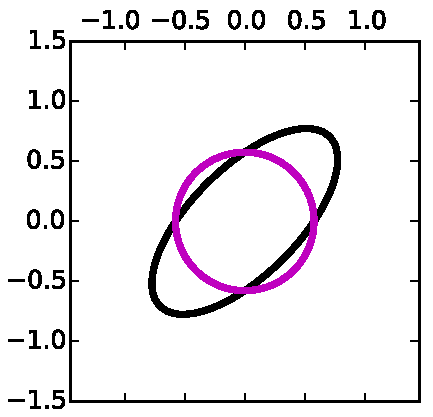
\includegraphics[width=0.25\linewidth]{Chapter2/vi/mean_field.pdf}
\caption{Mean-field approximation to the exact posterior distribution in the Bayesian linear regression example (with one-sigma contours). The exact posterior contour is shown in black and the variational approximation is in purple.}
\label{fig:chap2_mean_field}
\end{figure}


